\documentclass[tikz,border=6pt]{standalone}
% ---------------------------------------------------------------------------
%  VISUAL.tex  --  A lightweight visual atlas of the recurring patterns
%  (iso / dual / equiv) in the Dillon--Dobbertin formalisation library.
%  Minimal words; one TikZ picture per concept.  Compile page-by-page:
%      pdflatex VISUAL.tex        (standalone emits one PDF page per picture)
% ---------------------------------------------------------------------------
\usepackage{amsmath,amssymb}
\usetikzlibrary{arrows.meta,positioning,calc,decorations.pathreplacing,
                fit,backgrounds,shapes.geometric,decorations.markings}

\tikzset{
  grn/.style={draw=green!55!black,line width=.9pt,fill=green!12,rounded corners,
              font=\small,align=center,inner sep=4pt},
  gry/.style={draw=black!45,fill=black!4,rounded corners,font=\small,
              align=center,inner sep=4pt},
  ar/.style ={-{Stealth[length=2.4mm]},line width=.7pt},
  dar/.style={{Stealth[length=2.2mm]}-{Stealth[length=2.2mm]},line width=.7pt},
  dot/.style={circle,fill=black,inner sep=1.3pt},
  cdot/.style={circle,fill=blue!70!black,inner sep=1.6pt},
  lbl/.style={font=\footnotesize\itshape,text=black!60},
  hdr/.style={font=\small\bfseries},
}

\begin{document}

% ===========================================================================
% 1.  LAYERED IMPORT DAG  (the library as a rooted DAG; green = proven cores)
% ===========================================================================
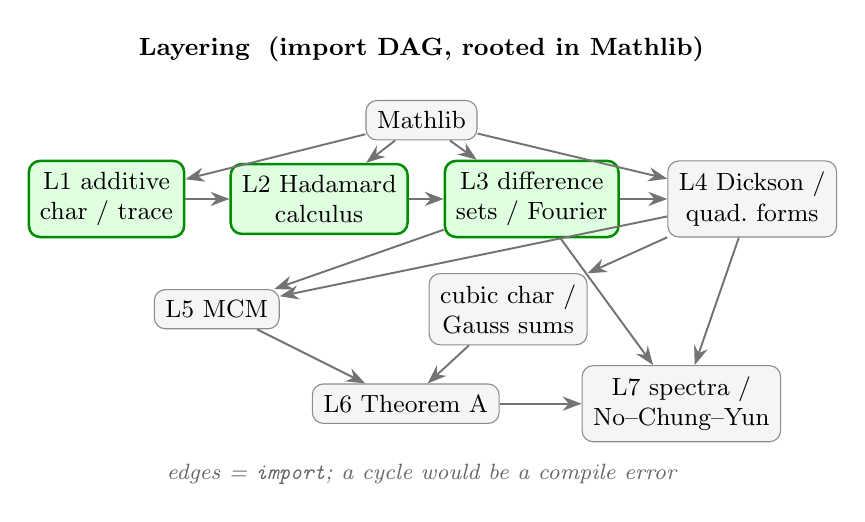
\begin{tikzpicture}[node distance=6mm and 10mm]
  \node[hdr] at (0,2.3) {Layering \;(import DAG, rooted in Mathlib)};
  \node[gry] (mlib) at (0,1.4) {Mathlib};
  \node[grn] (l1) at (-4,.4) {L1 additive\\char / trace};
  \node[grn] (l2) at (-1.3,.4) {L2 Hadamard\\calculus};
  \node[grn] (l3) at (1.4,.4) {L3 difference\\sets / Fourier};
  \node[gry] (l4) at (4.2,.4) {L4 Dickson /\\quad.\ forms};
  \node[gry] (mcm) at (-2.6,-1) {L5 MCM};
  \node[gry] (gs)  at (1.1,-1) {cubic char /\\Gauss sums};
  \node[gry] (main)at (-.2,-2.2) {L6 Theorem A};
  \node[gry] (spec)at (3.3,-2.2) {L7 spectra /\\No--Chung--Yun};
  \foreach \a/\b in {mlib/l1,mlib/l2,mlib/l3,mlib/l4,l1/l2,l2/l3,l3/l4,
                     l3/mcm,l4/mcm,l4/gs,mcm/main,gs/main,l3/spec,l4/spec,main/spec}
     \draw[ar,black!55] (\a)--(\b);
  \node[lbl] at (0,-3.1){edges = \texttt{import}; a cycle would be a compile error};
\end{tikzpicture}

% ===========================================================================
% 2.  DUALITY:  Hadamard transform is an involution  (F̂̂ = F)
% ===========================================================================
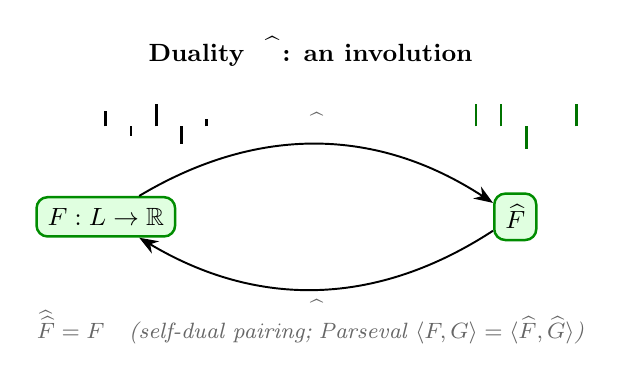
\begin{tikzpicture}
  \node[hdr] at (0,2.1){Duality \;$\widehat{\phantom{F}}$: an involution};
  \node[grn] (F) at (-2.6,0) {$F:L\to\mathbb R$};
  \node[grn] (Fh) at (2.6,0) {$\widehat F$};
  \draw[ar] (F) to[bend left=32] node[above,lbl]{$\widehat{\phantom{F}}$} (Fh);
  \draw[ar] (Fh) to[bend left=32] node[below,lbl]{$\widehat{\phantom{F}}$} (F);
  \node[lbl] at (0,-1.4){$\widehat{\widehat F}=F$\quad(self-dual pairing;\;Parseval $\langle F,G\rangle=\langle\widehat F,\widehat G\rangle$)};
  % small spectra glyphs
  \begin{scope}[shift={(-2.6,1.15)},scale=.32]
    \foreach \x/\h in {0/.6,1/-.4,2/.9,3/-.7,4/.3} \draw[line width=1pt](\x,0)--(\x,\h);
  \end{scope}
  \begin{scope}[shift={(2.1,1.15)},scale=.32]
    \foreach \x/\h in {0/.9,1/.9,2/-.9,3/.0,4/.9} \draw[line width=1pt,green!45!black](\x,0)--(\x,\h);
  \end{scope}
\end{tikzpicture}

% ===========================================================================
% 3.  EQUIVALENCE:  `Equivalent` is a groupoid; Arf invariant = colour class
% ===========================================================================
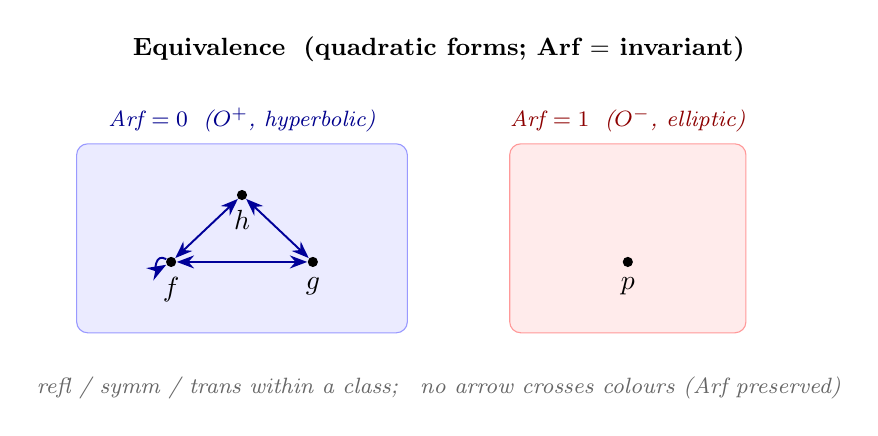
\begin{tikzpicture}
  \node[hdr] at (0,2.4){Equivalence \;(quadratic forms; Arf $=$ invariant)};
  % two colour classes
  \begin{scope}[on background layer]
    \node[draw=blue!40,fill=blue!8,rounded corners,minimum width=4.2cm,
          minimum height=2.4cm] (Aplus) at (-2.5,0){};
    \node[draw=red!40,fill=red!8,rounded corners,minimum width=3.0cm,
          minimum height=2.4cm] (Aminus) at (2.4,0){};
  \end{scope}
  \node[lbl,text=blue!55!black] at (-2.5,1.5){Arf $=0$ \;($O^{+}$, hyperbolic)};
  \node[lbl,text=red!55!black]  at (2.4,1.5){Arf $=1$ \;($O^{-}$, elliptic)};
  \node[dot,label=below:{$f$}] (f) at (-3.4,-.3){};
  \node[dot,label=below:{$g$}] (g) at (-1.6,-.3){};
  \node[dot,label=below:{$h$}] (h) at (-2.5,.55){};
  \node[dot,label=below:{$p$}] (p) at (2.4,-.3){};
  \draw[dar,blue!60!black] (f)--(g);
  \draw[dar,blue!60!black] (g)--(h);
  \draw[dar,blue!60!black] (f)--(h);
  \draw[ar,blue!60!black] (f) to[out=150,in=210,looseness=6] (f);
  \node[lbl] at (0,-1.9){refl / symm / trans within a class;\;
        \;no arrow crosses colours ($\text{Arf}$ preserved)};
\end{tikzpicture}

% ===========================================================================
% 4.  ISOMORPHISM:  cube classes  L*/(L*)^3  ≅  μ₃ ⊂ ℂ   (cubic character)
% ===========================================================================
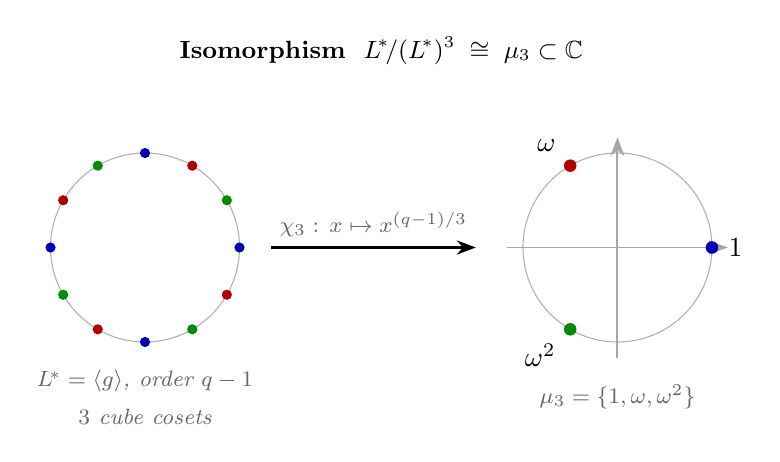
\begin{tikzpicture}[scale=1]
  \node[hdr] at (0,2.5){Isomorphism \;$L^{\!*}\!/(L^{\!*})^{3}\;\cong\;\mu_3\subset\mathbb C$};
  % left: cyclic group with 3 cosets
  \begin{scope}[shift={(-3,0)}]
    \draw[black!30] (0,0) circle (1.2);
    \foreach \k in {0,...,11}{
      \pgfmathtruncatemacro{\c}{mod(\k,3)}
      \definecolor{cc}{RGB}{0,0,0}
      \ifnum\c=0 \def\col{blue!70!black}\fi
      \ifnum\c=1 \def\col{red!70!black}\fi
      \ifnum\c=2 \def\col{green!55!black}\fi
      \node[dot,fill=\col] at ({90-30*\k}:1.2){};
    }
    \node[lbl] at (0,-1.7){$L^{\!*}=\langle g\rangle$, order $q-1$};
    \node[lbl] at (0,-2.15){$3$ cube cosets};
  \end{scope}
  % map
  \draw[ar,line width=1pt] (-1.4,0) -- node[above,lbl]{$\chi_3:\,x\mapsto x^{(q-1)/3}$} (1.2,0);
  % right: unit circle with cube roots of unity
  \begin{scope}[shift={(3,0)}]
    \draw[black!30] (0,0) circle (1.2);
    \draw[ar,black!35] (-1.4,0)--(1.4,0); \draw[ar,black!35](0,-1.4)--(0,1.4);
    \node[cdot,label=right:{$1$}] at (0:1.2){};
    \node[cdot,fill=red!70!black,label=above left:{$\omega$}] at (120:1.2){};
    \node[cdot,fill=green!55!black,label=below left:{$\omega^2$}] at (240:1.2){};
    \node[lbl] at (0,-1.9){$\mu_3=\{1,\omega,\omega^2\}$};
  \end{scope}
\end{tikzpicture}

% ===========================================================================
% 5.  AUTO / EQUIV:  multiplier  x ↦ x^t  conjugates translations
% ===========================================================================
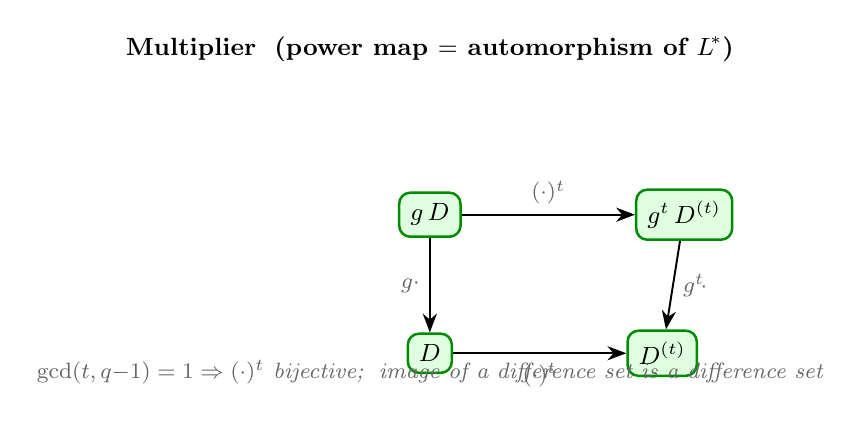
\begin{tikzpicture}[node distance=12mm and 22mm]
  \node[hdr] at (0,2.1){Multiplier \;(power map $=$ automorphism of $L^{\!*}$)};
  \node[grn] (gD)  {$g\,D$};
  \node[grn] (D)   [below=of gD] {$D$};
  \node[grn] (gtD) [right=of gD] {$g^{t}\,D^{(t)}$};
  \node[grn] (Dt)  [right=of D]  {$D^{(t)}$};
  \draw[ar] (gD) -- node[above,lbl]{$(\cdot)^t$} (gtD);
  \draw[ar] (D)  -- node[below,lbl]{$(\cdot)^t$} (Dt);
  \draw[ar] (gD) -- node[left,lbl]{$g\cdot$} (D);
  \draw[ar] (gtD)-- node[right,lbl]{$g^{t}\!\cdot$} (Dt);
  \node[lbl] at (0,-2.0){$\gcd(t,q{-}1)=1\Rightarrow (\cdot)^t$ bijective;\;
       image of a difference set is a difference set};
\end{tikzpicture}

% ===========================================================================
% 6.  PARTITION:  fibres of η partition L   (∑_v mult η v = q)
% ===========================================================================
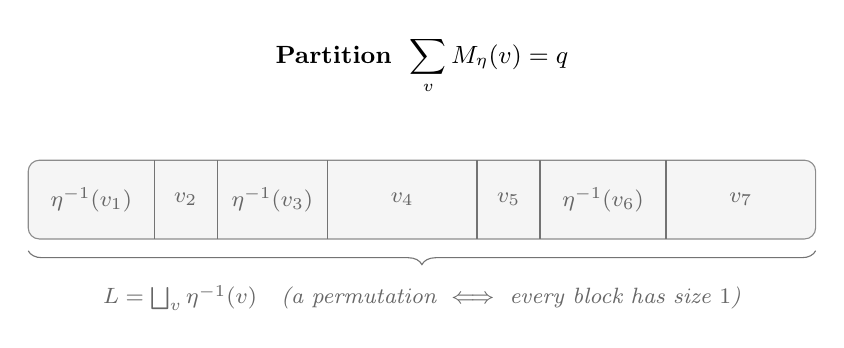
\begin{tikzpicture}
  \node[hdr] at (0,2.2){Partition \;$\displaystyle\sum_{v} M_\eta(v)=q$};
  \draw[gry,minimum width=1cm] (-5,0) rectangle (5,1);
  \def\xs{-5,-3.4,-2.6,-1.2,.7,1.5,3.1,5}
  \foreach \x in {-3.4,-2.6,-1.2,.7,1.5,3.1} \draw[black!55] (\x,0)--(\x,1);
  \node[lbl] at (-4.2,.5){$\eta^{-1}(v_1)$};
  \node[lbl] at (-3,.5){$v_2$};
  \node[lbl] at (-1.9,.5){$\eta^{-1}(v_3)$};
  \node[lbl] at (-.25,.5){$v_4$};
  \node[lbl] at (1.1,.5){$v_5$};
  \node[lbl] at (2.3,.5){$\eta^{-1}(v_6)$};
  \node[lbl] at (4.05,.5){$v_7$};
  \draw[decorate,decoration={brace,amplitude=5pt},black!55]
        (5,-.15)--(-5,-.15);
  \node[lbl] at (0,-.75){$L=\bigsqcup_v \eta^{-1}(v)$\quad(a permutation $\iff$ every block has size $1$)};
\end{tikzpicture}

% ===========================================================================
% 7.  DUALITY (Theorem B):  M̂_{f_k}(y) = M̂_{D_{2^k-1}}(y^{2^k+1})
% ===========================================================================
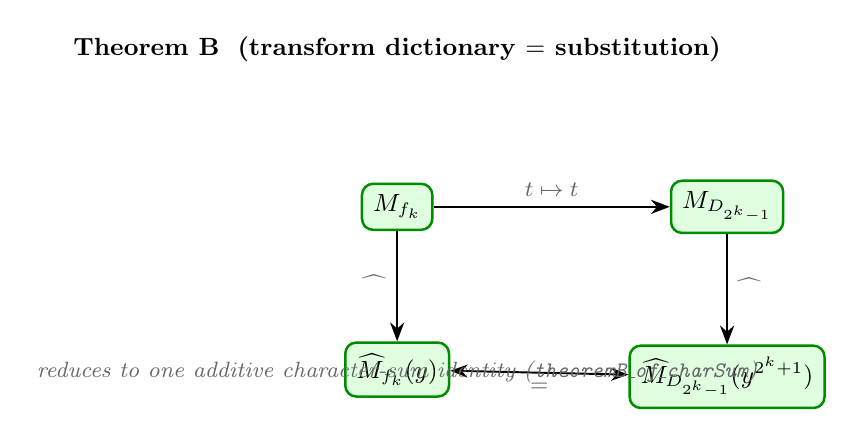
\begin{tikzpicture}[node distance=14mm and 30mm]
  \node[hdr] at (0,2.0){Theorem B \;(transform dictionary $=$ substitution)};
  \node[grn] (fk) {$M_{f_k}$};
  \node[grn] (D)  [right=of fk] {$M_{D_{2^k-1}}$};
  \node[grn] (fkh)[below=of fk] {$\widehat{M}_{f_k}(y)$};
  \node[grn] (Dh) [below=of D]  {$\widehat{M}_{D_{2^k-1}}(y^{2^k+1})$};
  \draw[ar] (fk)--node[above,lbl]{$t\mapsto t$}(D);
  \draw[ar] (fk)--node[left,lbl]{$\widehat{\phantom{M}}$}(fkh);
  \draw[ar] (D)--node[right,lbl]{$\widehat{\phantom{M}}$}(Dh);
  \draw[dar] (fkh)--node[below,lbl]{$=$}(Dh);
  \node[lbl] at (0,-2.1){reduces to one additive character-sum identity
        (\texttt{theoremB\_of\_charSum})};
\end{tikzpicture}

% ===========================================================================
% 8.  DUAL FOLDING:  Dickson  z ↦ z + z^{-1}  on the norm torus
% ===========================================================================
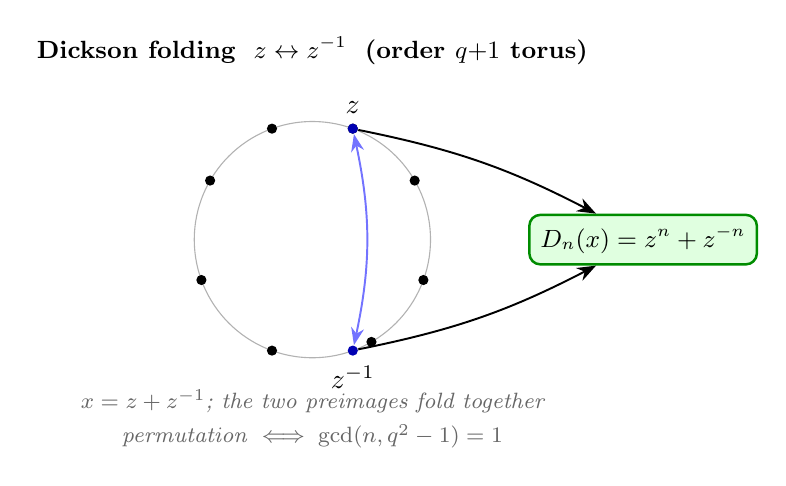
\begin{tikzpicture}
  \node[hdr] at (0,2.4){Dickson folding \;$z\leftrightarrow z^{-1}$ \;(order $q{+}1$ torus)};
  \draw[black!30] (0,0) circle (1.5);
  \foreach \a in {30,70,110,150,200,250,300,340}
     \node[dot] at (\a:1.5){};
  \node[dot,fill=blue!70!black,label=above:{$z$}] (z) at (70:1.5){};
  \node[dot,fill=blue!70!black,label=below:{$z^{-1}$}] (zi) at (-70:1.5){};
  \draw[dar,blue!55] (z) to[bend left=12] (zi);
  \node[grn] (val) at (4.2,0){$D_n(x)=z^n+z^{-n}$};
  \draw[ar] (z) to[bend left=8] node[above,lbl]{} (val);
  \draw[ar] (zi) to[bend right=8] (val);
  \node[lbl] at (0,-2.05){$x=z+z^{-1}$; the two preimages fold together};
  \node[lbl] at (0,-2.5){permutation $\iff \gcd(n,q^2-1)=1$};
\end{tikzpicture}

% ===========================================================================
% 9.  EQUIV CHAIN behind Theorem A  (Hadamard-equiv is transitive)
% ===========================================================================
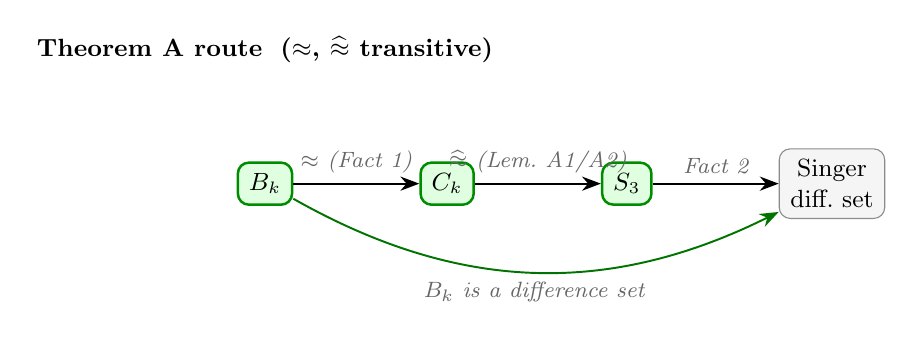
\begin{tikzpicture}[node distance=8mm and 16mm]
  \node[hdr] at (0,1.7){Theorem A route \;($\approx$, $\widehat\approx$ transitive)};
  \node[grn] (B) {$B_k$};
  \node[grn] (C) [right=of B]{$C_k$};
  \node[grn] (S) [right=of C]{$S_3$};
  \node[gry] (DS)[right=of S]{Singer\\diff.\ set};
  \draw[ar] (B)--node[above,lbl]{$\approx$ (Fact 1)}(C);
  \draw[ar] (C)--node[above,lbl]{$\widehat\approx$ (Lem.\ A1/A2)}(S);
  \draw[ar] (S)--node[above,lbl]{Fact 2}(DS);
  \draw[ar,green!45!black] (B) to[bend right=28] node[below,lbl]{$B_k$ is a difference set}(DS);
\end{tikzpicture}

\end{document}
